\documentclass{article} % For LaTeX2e
\usepackage{nips14submit_e,times}
\usepackage{amsmath}
\usepackage{amsthm}
\usepackage{amssymb}
\usepackage{mathtools}
\usepackage{hyperref}
\usepackage{url}
\usepackage{algorithm}
\usepackage[noend]{algpseudocode}
%\documentstyle[nips14submit_09,times,art10]{article} % For LaTeX 2.09

\usepackage{bbm}
\usepackage{graphicx}
\usepackage{caption}
\usepackage{subcaption}
\usepackage{MnSymbol}

\def\eQb#1\eQe{\begin{eqnarray*}#1\end{eqnarray*}}
\def\eQnb#1\eQne{\begin{eqnarray}#1\end{eqnarray}}
\providecommand{\e}[1]{\ensuremath{\times 10^{#1}}}
\providecommand{\pb}[0]{\pagebreak}
\DeclarePairedDelimiter\ceil{\lceil}{\rceil}
\DeclarePairedDelimiter\floor{\lfloor}{\rfloor}

\newcommand{\E}{\mathrm{E}}
\newcommand{\Var}{\mathrm{Var}}
\newcommand{\Cov}{\mathrm{Cov}}
\newcommand\eqD{\stackrel{\mathclap{\normalfont\mbox{d}}}{=}}

\def\Qb#1\Qe{\begin{question}#1\end{question}}
\def\Sb#1\Se{\begin{solution}#1\end{solution}}

\newenvironment{claim}[1]{\par\noindent\underline{Claim:}\space#1}{}
\newtheoremstyle{quest}{\topsep}{\topsep}{}{}{\bfseries}{}{ }{\thmname{#1}\thmnote{ #3}.}
\theoremstyle{quest}
\newtheorem*{definition}{Definition}
\newtheorem*{theorem}{Theorem}
\newtheorem*{lemma}{Lemma}
\newtheorem*{question}{Question}
\newtheorem*{preposition}{Preposition}
\newtheorem*{exercise}{Exercise}
\newtheorem*{challengeproblem}{Challenge Problem}
\newtheorem*{solution}{Solution}
\newtheorem*{remark}{Remark}
\usepackage{verbatimbox}
\usepackage{listings}
\usepackage{mathrsfs}
\title{ProbLimI: \\
Problem Set XI}


\author{
Youngduck Choi \\
CIMS \\
New York University\\
\texttt{yc1104@nyu.edu} \\
}


% The \author macro works with any number of authors. There are two commands
% used to separate the names and addresses of multiple authors: \And and \AND.
%
% Using \And between authors leaves it to \LaTeX{} to determine where to break
% the lines. Using \AND forces a linebreak at that point. So, if \LaTeX{}
% puts 3 of 4 authors names on the first line, and the last on the second
% line, try using \AND instead of \And before the third author name.

\newcommand{\fix}{\marginpar{FIX}}
\newcommand{\new}{\marginpar{NEW}}

\nipsfinalcopy % Uncomment for camera-ready version

\begin{document}


\maketitle

\begin{abstract}
This work contains solutions to the exercises of the problem set XI. The
chosen problems are 2,3,4.
\end{abstract}

\bigskip

\begin{question}[2]
\hfill
\begin{figure}[h!]
  \centering
    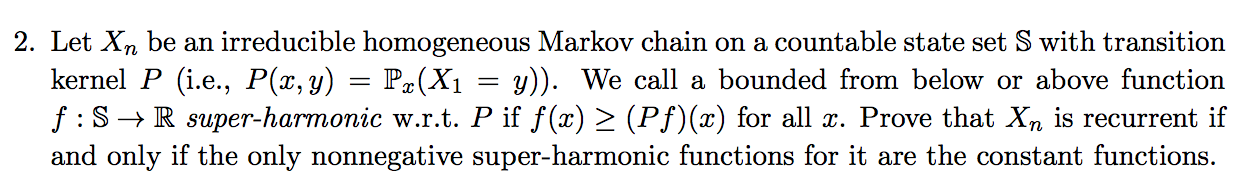
\includegraphics[width=0.7\textwidth]{prob-e11-p1.png}
\end{figure}
\end{question}
\begin{solution} \hfill \\
Observe that $f(X_n)$ is a super-martingale.
By martingale convergence, $f(X_n)$ converges a.s. to some RV $Y$. By 
recurrence, $Y = f(x)$ $\mathbb{P}_x$ a.s. so $f$ is constant.

Conversely, suppose the chain is transient. Define
\eQb
\tau &=& \inf\{ n \geq 0 : X_n = x_0 \}
\eQe
for some $x_0 \in \mathbb{S}$, and
\eQb
f(x) &=& \mathbb{P}(\tau < \infty \> | \> X_0 = x)
\eQe
By definition, $f(x) \in [0,1]$ for all $x$ and $f(x_0) = 1$.
By transience, $f(y) < 1$ for some $y \in \mathbb{S}$.
Observe that
\eQb
f(x) = \sum_{z \in \mathbb{S}} p(x,y)f(y)
\eQe
for all $x \in \mathbb{S}$, by strong markov property.
Hence, we have constructed a non-constant, super-harmonic function, and we are done.
\hfill $\qed$
 
\end{solution}

\newpage

\begin{question}[3]
\hfill
\begin{figure}[h!]
  \centering
    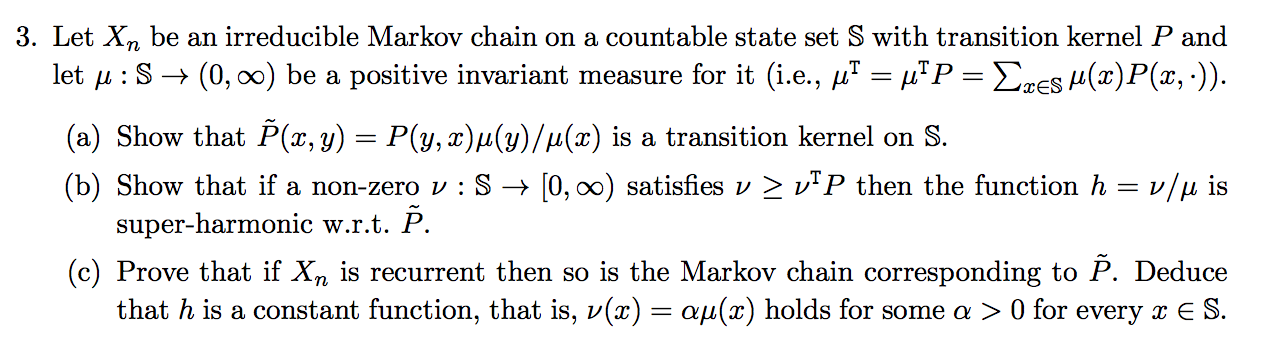
\includegraphics[width=0.7\textwidth]{prob-e11-p3.png}
\end{figure}
\end{question}
\begin{solution} \hfill \\
\textbf{(a)} As the space is discrete, we canonically equip it with the 
full sigma algebra, so 
\eQb
\tilde{P}(\cdot , A)
\eQe
is measurable for any $A \in 2^{\mathbb{S}}$. Furthermore,
\eQb
\tilde{P}(x,\cdot)
\eQe 
is a probability measure for any $x \in \mathbb{S}$, as
\eQb
\tilde{P}(x,\mathbb{S}) = \sum_{y \in \mathbb{S}} P(y,x)\mu(y) \mu(x)^{-1} =
\mu(x) \mu(x)^{-1} = 1 
\eQe
for any $x \in \mathbb{S}$, as $P$ is a transition kernel. Countable additivity
for each $x \in \mathbb{S}$ follows in the same way.

\textbf{(b)}
As $\nu \leq \nu^{T} P$, 
\eQb
h(y) \leq \sum_{s \in \mathbb{S}} h(x)\mu(x)P(x,y) = \sum_{s \in \mathbb{S}}
h(x) \mu(y) \tilde{P}(y,x) 
\eQe
for all $y \in \mathbb{S}$, so dividing both sides by $\mu(y)$, 
shows that $h$ is super-harmonic w.r.t $\tilde{P}$. 

\bigskip

\textbf{(c)}
From the same computation as $4-a$, we see that
\eQb
\tilde{P}^{n}(x,y) = \mu(y)\mu(x)^{-1}P^{n}(y,x)
\eQe
for all $x,y \in \mathbb{S}$. Hence, irreducibility and recurrency of $P$
implies that $\tilde{P}$ is irreducible and recurrent, since
\eQb
\sum_{n=1}^{\infty} P^{n}(x,x) = \infty = \sum_{n=1}^{\infty} \tilde{P}(x,x)  
\eQe
for any $x \in \mathbb{S}$.
Therefore,
by problem 2, $h$ is a constant function, and $\nu = \alpha \mu$ for some $\alpha > 0$.

\hfill $\qed$

\end{solution}

\newpage

\begin{question}[4]
\hfill
\begin{figure}[h!]
  \centering
    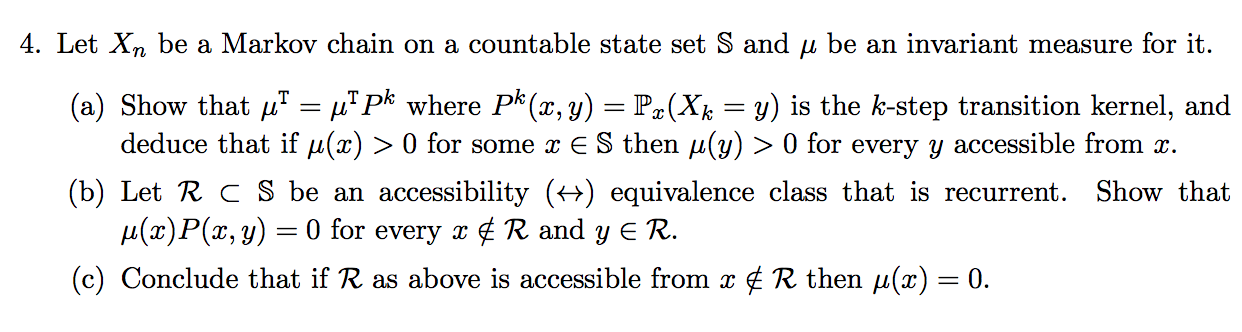
\includegraphics[width=0.7\textwidth]{prob-e11-p4.png}
\end{figure}
\end{question}
\begin{solution} \hfill \\
\textbf{(a)} When $n = 1$, the statement is true by definition of invariant
measure. Suppose the statement is true for some $n \geq 2$. Then, by fubini,
\eQb
\mu(x) &=& \sum_{s \in \mathbb{S}} \mu(s) P^{n}(s,x) 
= \sum_{t \in \mathbb{S}}\sum_{s \in \mathbb{S}} P^{n}(s,x) P(t,s) \\
&=& \sum_{t \in \mathbb{S}} P^{k}(t,x)\mu(t) 
\eQe 
for any $x \in \mathbb{S}$. Threrefore, by induction, we have the statement.

\smallskip

Suppose $\mu(x) > 0$, and let $y$ be accessible from $x$. Then, 
$p_{xy} > 0$, so $P^{n}(x,y) > 0$ for some $n$, as otherwise, by countable
subadditivity we have $p_{xy} = 0$, which is a contradiction.
Then, the above result,
\eQb
\mu(y) &=& \sum_{z \in \mathbb{S}} \mu(z)P^{n}(z,y) \geq \mu(x)P^{n}(x,y) > 0 
\eQe
as required.

\bigskip

\textbf{(b)} We provide the proof for the case when it's a stationary distribution.
Suppose $x$ is transient. Then, by the contrapositive of theorem 6.5.4 in Durrett,
$\mu(x) > 0$. Suppose $x$ is recurrent. Then, by theorem 6.4.3 in Durrett,
$p_{xy} = 0$, as otherwise $p_{yx} = 1$ and $x$ and $y$ communicate, which 
contradicts that $x \not\in R$. As $P(x,y) \leq p_{xy}$, $P(x,y) = 0$, and 
we are done. 

\bigskip

\textbf{(c)} If $R$ is accessible from $x \not\in R$, then $x$ must be transient.
Otherwise, by theorem 6.4.3, $p_{yx} = 1$, so $x$ and $y$ communicates, which 
is a contradiction. Therefore, as before $x$ being transient implies $\mu(x) > 0$. 

\hfill $\qed$

\end{solution}

\end{document}


